\part{Seminar 4 - Analytic Calculation of Eddy Currents in the Slots of Electrical Machines:
Application to Cage Rotor Induction Motors}

\makebox[.33\textwidth]{Morel Guillaume}\makebox[.33\textwidth]{Ramos Tornay Loris}\makebox[.33\textwidth]{Rase Arthur}


\section{Introduction}
This seminar is about the study of an induction machine. We develop in the next pages a model of a squirrel cage induction machine. This model, compare to a simulation by finite element, is useful to investigate the effect of the parameter of the machine on the torque and flux. 
\section{Description of the problem}
The main goal of the model is to get: first the field in the machine (it will induce the eddy current in the rotor thus the torque of the machine), second the torque of the machine (from Maxwell tensor) and third a collection of graph who display the behaviour of the machine. The study of the fields inside the machine are done in a 2D plane, see Figure \ref{fig:domaine}.
\subsection{Current sheet approximation}
This analysis of a induction machine (precisely the field inside it) is perform by considering a current flowing inside the stator winding. This current generate a flux inside the air gap. This same flux induce eddy current inside the squirrel cage. This methodology is the one used is the first course of \textit{convertisseur}.\\
In this paper, we want to derive the field inside the machine from partial differential equation point of view. This mean that we need boundary conditions. We thus use a representation of the current inside the stator winding known has : the current sheet approximation (see Figure \ref{fig:sheet}).
\begin{figure}[H]
    \centering
    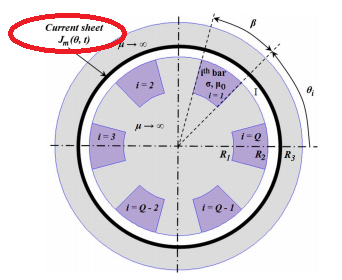
\includegraphics[scale=0.8]{currentSheet.png}
    \caption{Current sheet representation.}
    \label{fig:sheet}
\end{figure}
The expression of the current is written has : 
\begin{equation}
    J_{m} = \dfrac{3NI\sqrt{2}}{\pi R_{3}}K_{wm}cos(mp\theta_{s}-\omega_{s}t)
\end{equation}

\subsection{Winding factor}
the winding factor is the product of the pitch factor and the distribution factor : $K_{wm}=K_{p}K_{d}$. It represent the effect of the geometry of the machine on the field in the air gap :
\begin{itemize}
    \item pitch factor : represent the effect of the span (see slides) on the field generated.
    \item distribution factor : represent the influence of coupling multiple winding in a slot on the field.
\end{itemize}
They can be both quantify by the following expression : 
\begin{equation}
    K_{p}=sin\left(\dfrac{m\pi}{2}\right)sin\left(\dfrac{m\epsilon /\tau_{p}}{2}\right)
\end{equation}
\begin{equation}
    K_{d}=\dfrac{sin\left(\dfrac{mq\gamma}{2}\right)}{qsin\left(\dfrac{m\gamma}{2}\right)}
\end{equation}
\section{Computation of a model}
Now that we have our source term for the partial equation (the current $J_{m}$) we can use Maxwell equation's to compute a model that will give us the field in the machine.
\\
We use here 2 equations: Faraday's and Ampere's low,
\begin{equation}
    \nabla \times \textbf{E} = -\dfrac{\partial \textbf{B}}{\partial t}
\end{equation}
\begin{equation}
    \nabla \times \textbf{H} = \textbf{J} +\epsilon_{0}\dfrac{\partial \textbf{E}}{\partial t}
\end{equation}
If we use an analysis of the order of the equations, we can prove that the displacement current is negligible in the induction machine: 
\begin{equation}
    \text{Faraday: }\mathcal{O}(E/L) = \mathcal{O}(\mu_{0}H/\tau)
\end{equation}
\begin{equation}
    \text{Ampere: }\mathcal{O}(H_{erreur}/L) = \mathcal{O}(\epsilon_{0}E/\tau)
\end{equation}
where $L$ and $\tau$ are respectively the characteristic length and the characteristic time. The $H_{erreur}$ field, is the field where only the displacement current is taking into account. 
By doing the ratio of the real field and the approximated field ($H_{erreur}$) we get:
\begin{equation}
    \mathcal{O}(H_{erreur}/H) = \mathcal{O}(\epsilon_{0}\mu_{0}L^{2}/\tau^{2}) 
\end{equation}
We want this ratio to be has low has possible. This will mean that by neglecting the displacement current we don't make a big mistake in modeling the field in the machine with only the current density:
\begin{equation}
    \mathcal{O}(H_{erreur}/H)<<1 \Rightarrow \dfrac{L}{\tau}<< c
\end{equation}
with $c = \sqrt{\dfrac{1}{\mu_{0}\epsilon_{0}}}$ the speed of light. If we use the table in the reference paper, we can get a characteristic length and time to prove that:
\begin{equation}
    \dfrac{L}{\tau}<< c \Longleftrightarrow 2*10^{-10}<<2*10^{-2}
\end{equation}
We can conclude that the influence of the displacement current is negligible in front of the current density in the $H$ field (this is known has the MQS approximation):
\begin{equation}
    \boxed{\nabla \times \textbf{H} = \textbf{J}}
\end{equation}
Now, from this equation, we can use 3 thinks to get our model:
\begin{itemize}
    \item constitutive equation: $\textbf{J} = \sigma \textbf{E}$ (1)
    \item Faraday's law: $\nabla \times \textbf{E} = -\dfrac{\partial \textbf{B}}{\partial t}$ (2)
    \item vector identities: $\nabla(\nabla \cdot \textbf{A})-\nabla \times (\nabla \times \textbf{A}) = \nabla^{2}\textbf{A}$  (3)
\end{itemize}
These thinks will lead to the final model:
\begin{equation}
    \nabla \times \textbf{H} = \textbf{J}
\end{equation}
\begin{equation}
    \nabla \times (\nabla \times \textbf{A}) = \mu_{0}\textbf{J}
\end{equation}
with (3) and (1):
\begin{equation}\label{equation}
    \nabla(\nabla \cdot \textbf{A})- \nabla^{2}\textbf{A} = \mu_{0}\sigma\textbf{E}
\end{equation}
Using (2), we can "undo" the curl operation, and define a electric field:
\begin{equation}
    \nabla \times \textbf{E} = -\dfrac{\partial \textbf{B}}{\partial t}
\end{equation}
\begin{equation}
    \textbf{E} = -\dfrac{\partial \textbf{A}}{\partial t} - \nabla\phi
\end{equation}
by injecting this final result in equation (\ref{equation}) we get;
\begin{equation}
    \nabla(\nabla \cdot \textbf{A})- \nabla^{2}\textbf{A} = \mu_{0}\sigma\left(-\dfrac{\partial \textbf{A}}{\partial t} - \nabla\phi\right)
\end{equation}
The vector field $\textbf{A}$ is a field wich can be define from a reference potential. We finaly use the gauge transformation to perfom the last simplification: $A \longrightarrow A^{'} = A + \int \nabla \phi$, with the divergence set to 0\footnote{A physical meaning of this choice can be find in \textit{Introduction to electrodynamics, fouth edition} by David Griffiths}: $\nabla \cdot A^{'}=0$. Injecting this transformation in the last equation, we get Helmholtz's equation:
\begin{equation}
    \boxed{\nabla^{2}\textbf{A}^{'}=\mu_{0}\sigma_{0}\dfrac{\partial \textbf{A}^{'}}{\partial t}}
\end{equation}



\section{Analityc solution}
\subsection{Domain and boundary conditions}
We will start the analytic part of the seminar. For beginning, we must find the boundary conditions. So we need to define the domain. 
The first one is called i and the second Big I, as you can see on \ref{fig:domaine}.

\begin{figure}[H]
    \centering
    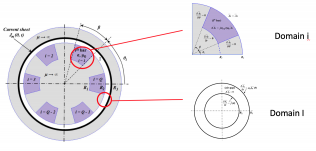
\includegraphics[scale=0.5]{domaine.png}
    \caption{Establishment of the domain}   
    \label{fig:domaine}
\end{figure}

We start the resolution with the domain i. Thanks to the use of the Maxwell's boundary conditions, the definition of B and the assumption :
\begin{eqnarray}\label{eq:0}
    \vec{n} \times (\vec{h_1}-\vec{h_2}) &=& \vec{J_s} \\
    \vec{B} &=& \mu \vec{H}\\
    \mu_{iron} &=& \infty
\end{eqnarray}

As said before the dependence of A is only in the z-direction , $A_i = A_i(r,\theta,t)e_z$. So by remplacing in the curl we have :

\begin{eqnarray}
    B &=& \nabla \times A\\
    B &=& \left[ \frac{1}{r} \frac{\partial A_z}{\partial \theta} - \frac{\partial A_\theta}{\partial z}\right]\hat{r}+ \left[ \frac{\partial A_r}{\partial z} - \frac{\partial A_z}{\partial r}\right]\hat{\theta}+\frac{1}{r} \left[ \frac{\partial}{\partial r}(rA_\theta ) - \frac{\partial A_r}{\partial \theta}\right]\hat{z}\\
\end{eqnarray}
    We have by simplification : 
\begin{equation}\label{eq:1}
    B = \left(\frac{1}{r} \frac{\partial A_z}{\partial \theta}\right)\hat{r}-\left(\frac{\partial A_z}{\partial r}\right)\hat{\theta}
\end{equation}
Now replacing Equation \ref{eq:1} in Equation \ref{eq:0} correspond to take the tangential component of the normal of each side. So for the radial component, see \ref{fig:domain2}, we have the following relation :

\begin{eqnarray}
    \frac{\partial\bar{A_i}}{\partial\theta}{\mid_{\theta = \theta_i}} = 0\\
    \frac{\partial\bar{A_i}}{\partial\theta}{\mid_{\theta = \theta_i+\beta}} = 0
\end{eqnarray}
And for the tangential : 
\begin{eqnarray}
\frac{\partial\bar{A_i}}{\partial r}{\mid_{r = R_1}} = 0
\end{eqnarray}

\begin{figure}[H]
    \centering
    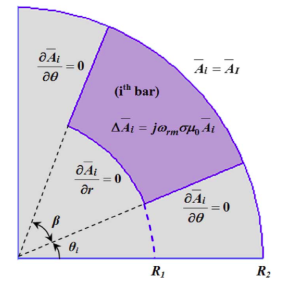
\includegraphics[scale=0.5]{domain2.png}
    \caption{Domain i}   
    \label{fig:domain2}
\end{figure}
\subsection{Helmoltz's equation: resolution}
Having all the boundary condition for this domain, we can continue. We begin to solve the Helmholtz's equation.
\begin{eqnarray}
\frac{\partial^2 \bar{A_i}}{\partial r^2} + \frac{1}{r} \frac{\partial \bar{A_i}}{\partial r} + \frac{1}{r^2}\frac{\partial^2 \bar{A_i}}{\partial \theta^2} = j \omega_{rm}\sigma\mu_0\bar{A_i}
\end{eqnarray}
Simply as we did in Math3, we use the method of separation of the variable :
\begin{eqnarray}
\bar{A}_i(r,\theta) = \rho_i(r) \Theta_i(\theta)
\end{eqnarray}
We have : 
\begin{eqnarray}
\bar{\Theta}_i" + \lambda \bar{\Theta}_i=0\\
r^2\bar{\rho_i"}+r\bar{\rho_i'}+(\alpha^2r^2-\lambda)\bar{\rho_i}=0
\end{eqnarray}
Where $ \alpha^2 = -j\omega_{rm} \sigma \mu_0 $
Resolving the first equation we have : 
\begin{eqnarray}
\bar{\Theta}_i" + \lambda \bar{\Theta}_i&=&0\\
\Theta &=& A cos[\sqrt\lambda(\Theta-\Theta_i)]+ B sin[\lambda(\Theta-\Theta_i)]\\
\frac{\partial \Theta}{\partial \theta} &=& - \sqrt{\lambda} A sin[\sqrt\lambda(\Theta-\Theta_i)]+ \lambda B cos[\lambda(\Theta-\Theta_i)]\\
\end{eqnarray}

Evaluate in $\theta \Rightarrow \theta_i = 0 $ and $\theta \Rightarrow \theta_i + \beta = 0 $ we have respectively :

\begin{eqnarray}
0 &=& \sqrt \lambda B  \\
0 &=& -\sqrt \lambda A sin[\sqrt \lambda \beta] 
\end{eqnarray}

We have finally the eigen-value and final solution for this part :

\begin{eqnarray}
\lambda_0 &=& 0\\
\lambda_k &=& \left( \frac{k\pi}{\beta}\right)^2 \\
\bar{\Theta}_{i0}(\theta) &=& 1\\
\bar{\Theta}_{ik}(\theta) &=& cos\left(\frac{k\pi}{\beta}(\theta-\theta_i)\right)
\end{eqnarray}

We will now continue with the second equation :
\begin{eqnarray}
r^2\bar{\rho_i"}+r\bar{\rho_i'}+(\alpha^2r^2-\lambda)\bar{\rho_i}&=&0
\end{eqnarray}
All of us know this equation \textbf{obviously}! It's the bessel's equation who has for solution :
\begin{eqnarray}
\bar{\rho}_{i0}(r) &=& \bar{A}_0^i J_0(\alpha r) + \bar{B}_0^iY_0(\alpha r)\\
\bar{\rho}_{ik}(r) &=& \bar{A}_k^i J_{k\pi/\beta}(\alpha r) + \bar{B}_{k}^iY_{k\pi/\beta}(\alpha r)
\end{eqnarray}

We have the two solutions of the two equation in this domain, we can multiplie this two and have :
\begin{eqnarray}\label{42}
\bar{A}_i(r,\theta) =  &\bar{A}_0^i J_0(\alpha r) + \bar{B}_0^i Y_0(\alpha r) + \\ 
& \sum_{k=1}^\infty \left( \bar{A}_k^i J_{k\pi/\beta}(\alpha r) + \bar{B}_k^i Y_{k\pi/\beta}(\alpha r) \right) cos\left( \frac{k\pi}{\beta} (\theta-\theta_i)\right)
\end{eqnarray}
The last thinks we have to do is imposed the last boundary condition. However some of this condition link the two domains, and we must solve the other domain before finishing the resolution.

\subsection{Laplace's equation: resolution}
Let's begin the resolution in the domain big I, see Figure \ref{fig:domain3}.
\begin{figure}[H]
    \centering
    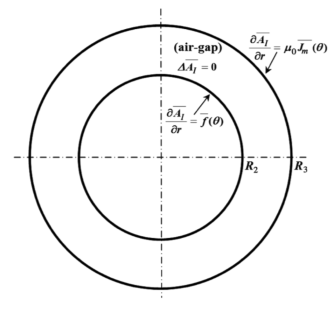
\includegraphics[scale=0.7]{domain3.png}
    \caption{Domain i}   
    \label{fig:domain3}
\end{figure}
The limit condition for this field will be find the like the same method of before. We have directly : 
\begin{eqnarray}
\frac{\partial\bar{A_I}}{\partial r}{\mid_{r = R_3}} &=& \mu_0 \bar{J}_m(\theta)\\
\frac{\partial\bar{A_I}}{\partial r}{\mid_{r = R_2}} &=& \bar{f}(\theta)\\
    \bar{f(\theta)}&=& 
\begin{cases}
    \frac{\partial \bar{A}_i}{\partial r}\mid_{r = R_2} &  \forall \theta \in [\theta_i,\theta_i+\beta]\\
    0               & \text{otherwise}
\end{cases}
\end{eqnarray}

For solve the equation is again with the method of separation of variables :
\begin{eqnarray}
\frac{\partial^2\bar{A}_I}{\partial r^2}+ \frac{1}{r}\frac{\partial\bar{A}_I}{\partial r}+\frac{1}{r^2}\frac{\partial^2 \bar{A}_I}{\partial \theta^2}&=&0\\
\bar{A}_I(r,\theta) &=& R_I(r) \Theta_I(\theta) \\
r^2R"+rR'-\lambda R &=& 0\\
\Theta"+\lambda\Theta &=& 0
\end{eqnarray}
Solving the two last equation give for the first the Laplace's solution and the same of before for the other :
\begin{eqnarray}
\Theta &=& A_n cos(n\theta) + B_n sin(n\theta)\\
R_n &=& C_n r^{n} + D_n r^{-n}
\end{eqnarray}
By multiplying :
\begin{eqnarray}
A(r,\theta) = &A_0 + \sum_{n=1}^\infty r^n(A_ncos(n\theta)\\
&+B_nsin(n\theta))+ \sum_{n=1}^\infty r^{-n}(C_ncos(n\theta)+D_nsin(n\theta))
\end{eqnarray}
And imposing the boundary conditions: 
\begin{eqnarray}
\bar{A}_I(r,\theta) = \bar{A}_0^I &+ \sum_{n=1}^\infty \left(\bar{A}_n^I\frac{R_2}{n}\frac{P_n(r,R_3)}{E_n(R_2,R_3)}+\bar{B}_n^I\frac{R_3}{n}\frac{P_n(r,R_2)}{E_n(R_3,R_2)}\right) cos(n\theta)\\
& + \sum_{n=1}^\infty \left(\bar{C}_n^I\frac{R_2}{n}\frac{P_n(r,R_3)}{E_n(R_2,R_3)}+\bar{D}_n^I\frac{R_3}{n}\frac{P_n(r,R_2)}{E_n(R_3,R_2)}\right) sin(n\theta)
\end{eqnarray}
Where we have :
\begin{eqnarray}
P_n(u,v) &=& \left(\frac{u}{v}\right)^n + \left(\frac{v}{u}\right)^n\\
E_n(u,v) &=& \left(\frac{u}{v}\right)^n - \left(\frac{v}{u}\right)^n\\
\bar{A}_n^I &=& \frac{2}{2\pi}\int_0^{2\pi} \bar{f}(\theta)cos(n\theta)d\theta\\
\bar{B}_n^I &=&\frac{2}{2\pi}\int_0^{2\pi} \mu_0\bar{J}_m(\theta)cos(n\theta)d\theta\\
\bar{C}_n^I &=& \frac{2}{2\pi}\int_0^{2\pi} \bar{f}(\theta)sin(n\theta)d\theta\\
\bar{D}_n^I &=& \frac{2}{2\pi}\int_0^{2\pi} \mu_0\bar{J}_m(\theta)sin(n\theta)d\theta
\end{eqnarray}
\subsection{Back to the Helmoltz's equation}
Now we have all to finish this part. We come back on the resolution of the helmholtz's equation. The boundary to apply for the last equation \ref{42} are the next one :

\begin{eqnarray}
\frac{\partial\bar{A_i}}{\partial r}{\mid_{r = R_1}} &=& 0\\
\bar{A}_i(R_2,\theta) &=& \bar{A}_I(R_2,\theta)
\end{eqnarray}

In fact, the second of this, correspond to the continuity of the two domaine.
Remember we have this relation :

\begin{eqnarray}
A &=& A(r,\theta,t)e_z\\
B &=& \left(\frac{1}{r} \frac{\partial A_z}{\partial \theta}\right)\hat{r}-\left(\frac{\partial A_z}{\partial r}\right)\hat{\theta}
\end{eqnarray}
And by applying the two condition of Maxwell : 
\begin{eqnarray}
\bar{n} \cdot (\bar{B}_1 - \bar{B}_2) &=& 0\\
\bar{n} \times (\bar{H}_1 - \bar{H}_2) &=& 0
\end{eqnarray}
It's lead to : 
\begin{eqnarray}
\frac{\partial A_i}{\partial \theta} &=& \frac{\partial A_I}{\partial \theta}\\
\frac{\partial A_i}{\partial r} &=& \frac{\partial A_I}{\partial r}
\end{eqnarray}
So :
\begin{eqnarray}
A_i &=& A_I + cst(\theta)\\
A_i &=& A_I + cst(r)
\end{eqnarray}
And the condition is find :
\begin{eqnarray}
\bar{A}_i(R_2,\theta) = \bar{A}_I(R_2,\theta)
\end{eqnarray}
Applying these conditions as said before gives :
\begin{eqnarray}
\bar{A}_i(r,\theta) = &\bar{C}_0^i\left( \frac{J_0(\alpha r) - \bar{F}_1Y_0(\alpha r)}{J_0(\alpha R_2) - \bar{F}_1Y_0(\alpha R_2)} \right )\\
&+ \sum_{k=1}^\infty \bar{C}_k^i \frac{J_{k\pi/\beta}(\alpha r) - \bar{F}_{k\pi/\beta}Y_{k\pi/\beta}(\alpha r)}{J_{k\pi/\beta}(\alpha R_2) - \bar{F}_{k\pi/\beta}Y_{k\pi/\beta}(\alpha R_2)} \\
& \times cos\left(\frac{k\pi}{\beta}(\theta-\theta_i)\right)
\end{eqnarray}
With :
\begin{eqnarray}
\bar{F}_1 &=& \frac{J_1(\alpha R_1)}{Y_1(\alpha R_1)}\\
\bar{F}_k &=& \frac{-\alpha J_{1+k\pi/\beta}(\alpha R_1) + \frac{k\pi}{\beta R_1}J_{k\pi/\beta}(\alpha R_1)}{-\alpha Y_{1+k\pi/\beta}(\alpha R_1) + \frac{k\pi}{\beta R_1}Y_{k\pi/\beta}(\alpha R_1)}\\
\bar{C}_0^i &=& \frac{1}{\beta} \int_{\theta_i}^{\theta_i+\beta} \bar{A}_I(R_2,\theta)d\theta\\
\bar{C}_k^i &=& \frac{2}{\beta} \int_{\theta_i}^{\theta_i+\beta} \bar{A}_I(R_2,\theta)cos\left(\frac{k\pi}{\beta}(\theta-\theta_i)\right)d\theta
\end{eqnarray}
We can then compute the magnetic field based on the expression of this potential vector with the equation computed previously.

Summary of this part :
\begin{itemize}
    \item Boundary condition of helmholtz’s equation 
    \item Solution of helmholtz’s equation
    \item Boundary condition of Laplace’s equation
    \item Solution of Laplace’s equation
    \item Come back to helmholtz’s equation
\end{itemize}

\section{Computation of the eddy currents}

We are now going to study the induced currents (eddy currents) in the slots of the machine. In order to find an expression of these currents, we develop the Ampere's law using the potential vector. We make the same assumption as we did previously: the displacement current is negligible compared to the current density. Introducing the second expression in the first one, we can obtain the current density: 
\begin{equation*}
   \nabla \times \overline{H} = \overline{J}
\end{equation*}
\begin{equation*}
    \overline{B} = \nabla \times \overline{A}
\end{equation*}
\begin{eqnarray}
\nabla \times \nabla \times \frac{\overline{A}}{\mu_0} &=& \overline{J}\\
\nabla (\nabla \cdot \overline{A}) - \Delta \overline{A} &=& \mu_0 \overline{J}
\end{eqnarray}
Using the results already explained before, we have: 
\begin{equation*}
    - \Delta \overline{A} = \mu_0 \overline{J}
\end{equation*}
And so, using the Helmoltz's equation: 
\begin{equation*}
    - \mu_0 \sigma\frac{\partial\overline{A}}{\partial t}  = \mu_0 \overline{J}
\end{equation*}
If we express this equation in the frequency domain, we finally have: 
\begin{equation*}
   \overline{J}_i =  - j \omega_{rm}  \sigma\frac{\partial\overline{A}}{\partial t} 
\end{equation*}

We have now to integrate the current density it in order to find the total current in each slot. We work with polar coordinates because of the shape of the slot. We still use the configuration shown at the beginning of section. 
\begin{equation}
I_i = \int_{R_1}^{R_2} \int_{\theta_i}^{\theta_i+\beta} J_i(r,\theta) \hspace{1mm} r dr d\theta
\end{equation}
If we substitute the expression of the potential vector we found previously, we obtain: 
$$
{\scriptstyle
I_i = \int_{R_1}^{R_2} \int_{\theta_i}^{\theta_i+\beta} -j \omega_{rm} \sigma \Bigg( \overline{C_0^i} \frac{J_0(\alpha r) - \overline{F_1} Y_0(\alpha r)}{J_0( \alpha R_2) - \overline{F_1} Y_0(\alpha R_2)} + \sum_{k=1}^{\infty} \overline{C_k^i} \frac{J_{k \pi / \beta}(\alpha r) - \overline{F_k} Y_{k \pi / \beta}(\alpha r)}{J_{k \pi / \beta}( \alpha R_2) - \overline{F_k} Y_{k \pi / \beta}(\alpha R_2)}  cos(\frac{k \pi}{\beta} (\theta - \theta_i) \Bigg) r dr d\theta}
$$
We have two terms. If we develop the second term, we can see the integral of the cosine is null. It remains only the first term:
\begin{equation*}
\int_{R_1}^{R_2} \int_{\theta_i}^{\theta_i+\beta} -j \omega_{rm} \sigma \Bigg( \overline{C_0^i} \frac{J_0(\alpha r) - \overline{F_1} Y_0(\alpha r)}{J_0( \alpha R_2) - \overline{F_1} Y_0(\alpha R_2)}  \Bigg) r dr d\theta
\end{equation*}
We can separate this term into two integrals and simplify them by putting all the constant terms outside the integrals:
\begin{equation*}
\frac{-j \omega_{rm} \sigma \overline{C_0^i}}{J_0( \alpha R_2) - \overline{F_1} Y_0(\alpha R_2)} \int_{R_1}^{R_2}   \Bigg(  J_0(\alpha r) - \overline{F_1} Y_0(\alpha r)  \Bigg) r dr \int_{\theta_i}^{\theta_i+\beta} 1 \hspace{1mm}d\theta
\end{equation*}
The second factor is simply equal to $\beta$. We know study the first part. Using the following Bessel functions property we can find the second expression:
\begin{equation*}
    \frac{d}{dx} (x \hspace{1mm} J_1(x))  = x \hspace{1mm} J_0(x)
\end{equation*}
\begin{equation*}
\frac{-j \omega_{rm} \sigma \overline{C_0^i}}{J_0( \alpha R_2) - \overline{F_1} Y_0(\alpha R_2)} \frac{\beta}{\alpha}   \Bigg(  R_2 \hspace{1mm} J_1(\alpha R_2) - \overline{F_1}\hspace{1mm}R_2 \hspace{1mm}Y_1(\alpha R_2) - \Big( R_1 \hspace{1mm} J_1(\alpha R_1) - \overline{F_1}\hspace{1mm}R_1 \hspace{1mm}Y_1(\alpha R_1) \Big) \Bigg)  
\end{equation*}
And so the final expression of the current in the ith slot is:
\begin{equation*}
\overline{I_i} = \frac{j \omega_{rm} \sigma \overline{C_0^i} \beta R_2}{\alpha}   \Bigg( \frac{J_1(\alpha R_1)\hspace{1mm}Y_1(\alpha R_2) - J_1(\alpha R_2)\hspace{1mm}Y_1(\alpha R_1)} {J_0(\alpha R_2)\hspace{1mm}Y_1(\alpha R_1) - J_1(\alpha R_1)\hspace{1mm}Y_0(\alpha R_2)} \Bigg)  
\end{equation*}


\section{Computation of the electromagnetic torque}
In this section, we are going to compute the electromagnetic torque based on the magnetic field established in the machine. In order to do that, we first compute the resultant force in the machine and then, using the definition of the torque, we will compute it.

To compute the total force, we use a force per volume that we then integrate. This force is computed from the Lorentz force per volume and the Ampere's law. Combining these two expressions allows to find an expression of the force that depends only on the magnetic field:
\begin{eqnarray*}
\overline{f} &=&  \overline{J} \times \overline{B}
\end{eqnarray*}
\begin{equation*}
\nabla \times \overline{H} = \overline{J} 
\end{equation*}
\begin{eqnarray*}
\overline{f} &=& \frac{1}{\mu_0} (\nabla \times \overline{B}) \times \overline{B}\\
 &=& -\hspace{3mm}\frac{1}{\mu_0} \overline{B}\times  (\nabla \times \overline{B}) 
\end{eqnarray*}
We know the Gauss's law of magnetism $\nabla \cdot \overline{B} = 0$. This allows to add a new term which is null in order to find a certain symmetry in the expression of the force. Using results from vectorial analysis and Gauss's law for magnetism gives:
\begin{equation*}
\overline{f} = \frac{1}{\mu_0} \Big((\nabla \cdot \overline{B}) \overline{B}   + (\overline{B} \cdot \nabla) \overline{B}  ) \Big) - \frac{1}{2\mu_0} \nabla(B^2)
\end{equation*}
We can now introduce the Maxwell stress tensor:
\begin{equation*}
 \sigma_{ij} = \frac{1}{\mu_0} \Big(B_i B_j - \frac{1}{2} \delta_{ij} B^2 \Big)
\end{equation*}
such as:
\begin{equation*}
\overline{f} = \nabla \cdot \sigma_{ij}
\end{equation*}
As supposed at the beginning of the seminar $ B_z = 0$ and so we can express the tensor as a matrix:
\[ \sigma_{ij} =  \frac{1}{\mu_0}\left( \begin{array}{ccc}
\frac{B_{r}^{2}-B_{\theta}^{2}}{2} & B_{r}B_{\theta}& 0 \\
B_{\theta} B_{r} &  \frac{B_{\theta}^{2}-B_{r}^{2}}{2} &  0 \\
0 & 0  & -\frac{B_{r}^{2}+B_{\theta}^{2}}{2} \end{array} \right) \]
Now we have computed the force per volume through the Maxwell stress tensor, we can now compute the total force and the electromagentic torque. We can integrate the force per volume and find the total force using the divergence theorem:
\begin{eqnarray*}
\overline{F} &=& \iiint_V \nabla \cdot \sigma_{ij} \hspace{4mm} dV\\
 &=& \oiint_S \sigma_{ij} \cdot \hat{n} \hspace{4mm} dS
\end{eqnarray*}
We have an integral over a closed surface. We choose for that a cylindar contained in the airgap. But the expression of the force per volume doesn't depend on z and so the products $\sigma_{ij} \cdot \hat{n}$ along the normal of each circular surfaces are opposite and cancel each other. It remains only the integration over the lateral surface:
\[
    \overline{F} = \frac{1}{\mu_0} \iint_{S,side} \Big(\frac{B_{r}^{2}-B_{\theta}^{2}}{2}\hspace{1mm}  \hat{e}_{r}  + B_{\theta} B_{r}\hspace{1mm}  \hat{e}_{\theta}\Big) \hspace{4mm} dS
\]
We can finally find the torque as:
\begin{eqnarray*}
    T_e &=& \hat{r} \times \overline{F}\\
    &=& R_e \hspace{1mm}  \hat{e}_{r} \times \frac{1}{\mu_0} \int_{0}^{L} \int_{0}^{2 \pi}  \Big(\frac{B_{r}^{2}(R_e,\theta)-B_{\theta}^{2}(R_e,\theta)}{2}\hspace{1mm}  \hat{e}_{r}  + B_{\theta}(R_e,\theta) B_{r}(R_e,\theta)\hspace{1mm}  \hat{e}_{\theta}\Big) \hspace{4mm} R_e d\theta \hspace{1mm} dL
\end{eqnarray*}
Developing it and expressing it with complex numbers (as the calculation is complex) gives:
\begin{equation*}
    T_e = \frac{L R_{e}^{2}}{\mu_0} \int_{0}^{2 \pi}  Re \Big[B_{\theta}(R_e,\theta) B_{r}^{*}(R_e,\theta)\hspace{1mm}  \hat{e}_{z}\Big] \hspace{4mm} d\theta
\end{equation*}
We can then introduce the expression of the magnetic field B in the previous equation and find a final expression of the torque.
\section{Results}
In this section, we are going to show some results obtained that shows the effectiveness of the model.

\subsection{Hypotheses}
\begin{itemize}
    \item full pitch stator winding
    \begin{equation*}
\lambda = \pi
\end{equation*}

\begin{equation*}
sin(|m| \pi/2) \hspace{1mm} sin(|m| \lambda/2) = 1 
\end{equation*}

\item One slot per pole per phase
\begin{equation*}
q = 1
\end{equation*}

\begin{equation*}
\frac{sin(|m| \pi/6)}{q\hspace{1mm} sin(|m| \pi/6q)}   = 1 
\end{equation*}

\item Small slot opening
\begin{equation*}
\epsilon \simeq 0
\end{equation*}

\begin{equation*}
\frac{sin(|m| \epsilon/2)}{|m| \epsilon/2}   \simeq 1 
\end{equation*}

\end{itemize}

And so the winding facor is equal to 1.

\subsection{Results for the fundamental component of of the stator curent sheet}

\subsubsection{Under no load condition}
We can see on the Figure \ref{fig:no-load} the magnetic field is mainly radial but we have a non-zero tangential component. The two components have a sinusoidal distribution over the rotor. We can see we have drops around the slots. This is due to the increased reluctance because of the airgap which leads to a decreasing magnetic flux. 
\begin{figure}[H]
    \begin{minipage}{.3 \textwidth}
        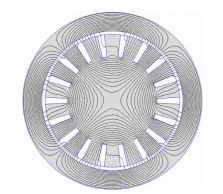
\includegraphics[scale=0.4]{graphe2.png}
    \end{minipage}
    \begin{minipage}{.3 \textwidth}
        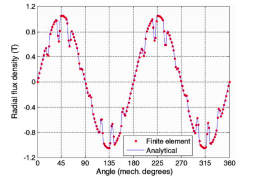
\includegraphics[scale=0.3]{graphe1.png}
        
    \end{minipage}
    \begin{minipage}{.3 \textwidth}
        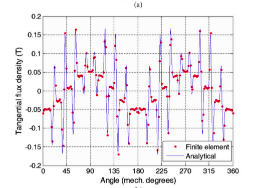
\includegraphics[scale=0.3]{graphe3.png}
    \end{minipage}
    \caption{Machine under no load condition}
    \label{fig:no-load}
    
\end{figure}
\subsubsection{Under locked-rotor condition}
We can see on the Figure \ref{fig:locked} we have much less radial flux and more flux closed loop in the airgap. We can also see the currents in the slots symbolised by the color on the picture. We can see these currents are not constant, we have perturbations due to the skin effect and the phase of the currents. The skin effect "pushes" the current at the boundary of the carrier slot. But there is a second effect, the phase of the current, which causes the peak of current to "sink" into the slots because of the phase shifting of these currents.

\begin{figure}[H]
    \begin{minipage}{.3 \textwidth}
        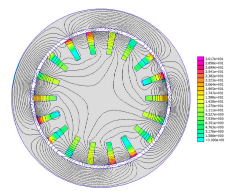
\includegraphics[scale=0.3]{graphe4.png}
    \end{minipage}
    \begin{minipage}{.3 \textwidth}
        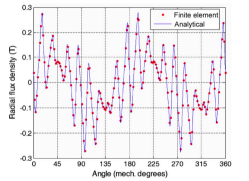
\includegraphics[scale=0.3]{graphe5.png}
        
    \end{minipage}
    \begin{minipage}{.3 \textwidth}
        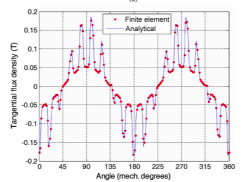
\includegraphics[scale=0.3]{graphe6.png}
    \end{minipage}
    \caption{Machine under locked-rotor condition}
    \label{fig:locked}
    
\end{figure}
We can see on the Figure \ref{fig:locked2} the currents have a sinusoidal distribution at each moment. We can see on the first picture the effect of the skin effect which increases the amount of current at the boundary of the slot. The last picture shows the well-known and expected torque-slip curve centred around 0 because we have only the fundamental component of the stator current. 
\begin{figure}[H]
    \begin{minipage}{.3 \textwidth}
        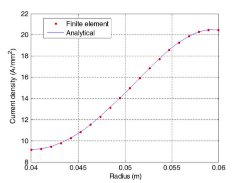
\includegraphics[scale=0.3]{graphe7.png}
    \end{minipage}
    \begin{minipage}{.3 \textwidth}
        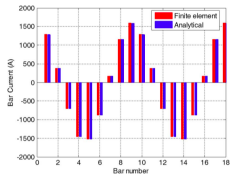
\includegraphics[scale=0.3]{graphe8.png}
        
    \end{minipage}
    \begin{minipage}{.3 \textwidth}
        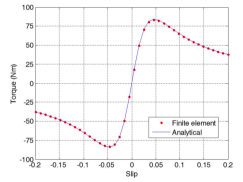
\includegraphics[scale=0.3]{graphe9.png}
    \end{minipage}
    \caption{Torque and currents for a machine under locked-rotor condition}
    \label{fig:locked2}
    
\end{figure}



\subsection{Results for the 5th harmonic of the stator curent sheet with locked-rotor condition}

We can see on the Figure \ref{fig:5th} we have the same results as for the fundamental component of the stator current but with lower intensities. We still have perturbations due to skin and phase effects. The second picture shows these effects. The peak is due to the skin effect. But it is not at the boundary of the slot because of the phase shifting of the current among successive slots which make the peak sinking deeper into the slots. On the third picture, we can see the torque-slip curve which is centred around 1.2 now because we are working with the 5th harmonic. 
\begin{figure}[H]
    \begin{minipage}{.3 \textwidth}
        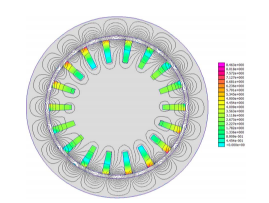
\includegraphics[scale=0.3]{graphe10.png}
    \end{minipage}
    \begin{minipage}{.3 \textwidth}
        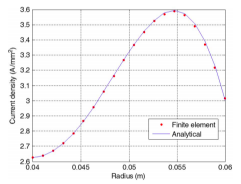
\includegraphics[scale=0.35]{graphe13.png}
        
    \end{minipage}
    \begin{minipage}{.3 \textwidth}
        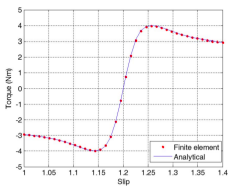
\includegraphics[scale=0.35]{graphe15.png}
    \end{minipage}
    \caption{Machine under locked-rotor condition (5th harmonic)}
    \label{fig:5th}
\end{figure}

\subsection{Torque due to the fundamental with 5th and 7th space harmonic effects}
We can see on the Figure \ref{fig:total_torque} the torque due to the fundamental component of the current sheet disturbed by the effects of the 5th and 7th harmonics. The blue curve is the one of the fundamental. It is the same that was shown before but we only have the right part her. We can observe the this the main responsible of the total torque. But we have two perturbations due to the harmonics. For example, we can see we have an important oscillation around s=1.2 because of the shape of the torque-slip curve due to the 5th harmonics. So the current applied by the current sheet at the stator can have parasitic effects on the thorque generation.
\begin{figure}[H]
    \centering
    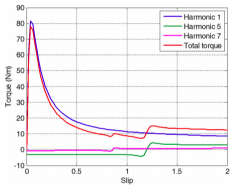
\includegraphics[scale=0.7]{graphe16.png}
    \caption{Torque for the 1st, 5th and 7th harmonics}
    \label{fig:total_torque}
\end{figure}
